% =============== Set the basic ============== %
\documentclass[10pt, xcolor={dvipsnames,x11names},compress]{beamer}
\usepackage{tikz}
\usepackage{tabulary}
\usepackage{algorithm,algpseudocode}
\usepackage{etoolbox}
\usepackage{booktabs}
\usepackage{amssymb}
\usepackage{amsfonts}
\usepackage{amsthm}
\usepackage{bm}
\usepackage{float}
\usepackage{graphicx}
\usepackage{mwe}
\usepackage{siunitx}
\usepackage{hyperref}
\usepackage{biblatex}
\addbibresource{main.bib}
\usecolortheme{spruce}
\useoutertheme{infolines}
\usefonttheme[onlymath]{serif}
\setbeamertemplate{headline}[default]
\setbeamertemplate{navigation symbols}{}
\mode<beamer>{\setbeamertemplate{blocks}[rounded][shadow=true]}
\setbeamercovered{transparent}
%%%%% NEW MATH DEFINITIONS %%%%%
\usepackage{etoolbox}
\usepackage{amsmath,amsfonts,bm}

% Mark sections of captions for referring to divisions of figures
\newcommand{\figleft}{{\em (Left)}}
\newcommand{\figcenter}{{\em (Center)}}
\newcommand{\figright}{{\em (Right)}}
\newcommand{\figtop}{{\em (Top)}}
\newcommand{\figbottom}{{\em (Bottom)}}
\newcommand{\captiona}{{\em (a)}}
\newcommand{\captionb}{{\em (b)}}
\newcommand{\captionc}{{\em (c)}}
\newcommand{\captiond}{{\em (d)}}

% Highlight a newly defined term
\newcommand{\newterm}[1]{{\bf #1}}


% Figure reference, lower-case.
\def\figref#1{figure~\ref{#1}}
% Figure reference, capital. For start of sentence
\def\Figref#1{Figure~\ref{#1}}
\def\twofigref#1#2{figures \ref{#1} and \ref{#2}}
\def\quadfigref#1#2#3#4{figures \ref{#1}, \ref{#2}, \ref{#3} and \ref{#4}}
% Section reference, lower-case.
\def\secref#1{section~\ref{#1}}
% Section reference, capital.
\def\Secref#1{Section~\ref{#1}}
% Reference to two sections.
\def\twosecrefs#1#2{sections \ref{#1} and \ref{#2}}
% Reference to three sections.
\def\secrefs#1#2#3{sections \ref{#1}, \ref{#2} and \ref{#3}}
% Reference to an equation, lower-case.
\def\eqref#1{equation~\ref{#1}}
% Reference to an equation, upper case
\def\Eqref#1{Equation~\ref{#1}}
% A raw reference to an equation---avoid using if possible
\def\plaineqref#1{\ref{#1}}
% Reference to a chapter, lower-case.
\def\chapref#1{chapter~\ref{#1}}
% Reference to an equation, upper case.
\def\Chapref#1{Chapter~\ref{#1}}
% Reference to a range of chapters
\def\rangechapref#1#2{chapters\ref{#1}--\ref{#2}}
% Reference to an algorithm, lower-case.
\def\algref#1{algorithm~\ref{#1}}
% Reference to an algorithm, upper case.
\def\Algref#1{Algorithm~\ref{#1}}
\def\twoalgref#1#2{algorithms \ref{#1} and \ref{#2}}
\def\Twoalgref#1#2{Algorithms \ref{#1} and \ref{#2}}
% Reference to a part, lower case
\def\partref#1{part~\ref{#1}}
% Reference to a part, upper case
\def\Partref#1{Part~\ref{#1}}
\def\twopartref#1#2{parts \ref{#1} and \ref{#2}}

\def\ceil#1{\lceil #1 \rceil}
\def\floor#1{\lfloor #1 \rfloor}
\def\1{\bm{1}}
\newcommand{\train}{\mathcal{D}}
\newcommand{\valid}{\mathcal{D_{\mathrm{valid}}}}
\newcommand{\test}{\mathcal{D_{\mathrm{test}}}}

\def\eps{{\epsilon}}


% Random variables
\def\reta{{\textnormal{$\eta$}}}
\def\ra{{\textnormal{a}}}
\def\rb{{\textnormal{b}}}
\def\rc{{\textnormal{c}}}
\def\rd{{\textnormal{d}}}
\def\re{{\textnormal{e}}}
\def\rf{{\textnormal{f}}}
\def\rg{{\textnormal{g}}}
\def\rh{{\textnormal{h}}}
\def\ri{{\textnormal{i}}}
\def\rj{{\textnormal{j}}}
\def\rk{{\textnormal{k}}}
\def\rl{{\textnormal{l}}}
% rm is already a command, just don't name any random variables m
\def\rn{{\textnormal{n}}}
\def\ro{{\textnormal{o}}}
\def\rp{{\textnormal{p}}}
\def\rq{{\textnormal{q}}}
\def\rr{{\textnormal{r}}}
\def\rs{{\textnormal{s}}}
\def\rt{{\textnormal{t}}}
\def\ru{{\textnormal{u}}}
\def\rv{{\textnormal{v}}}
\def\rw{{\textnormal{w}}}
\def\rx{{\textnormal{x}}}
\def\ry{{\textnormal{y}}}
\def\rz{{\textnormal{z}}}

% Random vectors
\def\rvepsilon{{\mathbf{\epsilon}}}
% \def\rvtheta{{\mathbf{\theta}}}
\def\boldtheta{{\boldsymbol{\theta}}}
\def\boldalpha{{\boldsymbol{\alpha}}}
\def\boldbeta{{\boldsymbol{\beta}}}
\def\rva{{\mathbf{a}}}
\def\rvb{{\mathbf{b}}}
\def\rvc{{\mathbf{c}}}
\def\rvd{{\mathbf{d}}}
\def\rve{{\mathbf{e}}}
\def\rvf{{\mathbf{f}}}
\def\rvg{{\mathbf{g}}}
\def\rvh{{\mathbf{h}}}
\def\rvu{{\mathbf{i}}}
\def\rvj{{\mathbf{j}}}
\def\rvk{{\mathbf{k}}}
\def\rvl{{\mathbf{l}}}
\def\rvm{{\mathbf{m}}}
\def\rvn{{\mathbf{n}}}
\def\rvo{{\mathbf{o}}}
\def\rvp{{\mathbf{p}}}
\def\rvq{{\mathbf{q}}}
\def\rvr{{\mathbf{r}}}
\def\rvs{{\mathbf{s}}}
\def\rvt{{\mathbf{t}}}
\def\rvu{{\mathbf{u}}}
\def\rvv{{\mathbf{v}}}
\def\rvw{{\mathbf{w}}}
\def\rvx{{\mathbf{x}}}
\def\rvy{{\mathbf{y}}}
\def\rvz{{\mathbf{z}}}

% Elements of random vectors
\def\erva{{\textnormal{a}}}
\def\ervb{{\textnormal{b}}}
\def\ervc{{\textnormal{c}}}
\def\ervd{{\textnormal{d}}}
\def\erve{{\textnormal{e}}}
\def\ervf{{\textnormal{f}}}
\def\ervg{{\textnormal{g}}}
\def\ervh{{\textnormal{h}}}
\def\ervi{{\textnormal{i}}}
\def\ervj{{\textnormal{j}}}
\def\ervk{{\textnormal{k}}}
\def\ervl{{\textnormal{l}}}
\def\ervm{{\textnormal{m}}}
\def\ervn{{\textnormal{n}}}
\def\ervo{{\textnormal{o}}}
\def\ervp{{\textnormal{p}}}
\def\ervq{{\textnormal{q}}}
\def\ervr{{\textnormal{r}}}
\def\ervs{{\textnormal{s}}}
\def\ervt{{\textnormal{t}}}
\def\ervu{{\textnormal{u}}}
\def\ervv{{\textnormal{v}}}
\def\ervw{{\textnormal{w}}}
\def\ervx{{\textnormal{x}}}
\def\ervy{{\textnormal{y}}}
\def\ervz{{\textnormal{z}}}

% Random matrices
\def\rmA{{\mathbf{A}}}
\def\rmB{{\mathbf{B}}}
\def\rmC{{\mathbf{C}}}
\def\rmD{{\mathbf{D}}}
\def\rmE{{\mathbf{E}}}
\def\rmF{{\mathbf{F}}}
\def\rmG{{\mathbf{G}}}
\def\rmH{{\mathbf{H}}}
\def\rmI{{\mathbf{I}}}
\def\rmJ{{\mathbf{J}}}
\def\rmK{{\mathbf{K}}}
\def\rmL{{\mathbf{L}}}
\def\rmM{{\mathbf{M}}}
\def\rmN{{\mathbf{N}}}
\def\rmO{{\mathbf{O}}}
\def\rmP{{\mathbf{P}}}
\def\rmQ{{\mathbf{Q}}}
\def\rmR{{\mathbf{R}}}
\def\rmS{{\mathbf{S}}}
\def\rmT{{\mathbf{T}}}
\def\rmU{{\mathbf{U}}}
\def\rmV{{\mathbf{V}}}
\def\rmW{{\mathbf{W}}}
\def\rmX{{\mathbf{X}}}
\def\rmY{{\mathbf{Y}}}
\def\rmZ{{\mathbf{Z}}}

% Elements of random matrices
\def\ermA{{\textnormal{A}}}
\def\ermB{{\textnormal{B}}}
\def\ermC{{\textnormal{C}}}
\def\ermD{{\textnormal{D}}}
\def\ermE{{\textnormal{E}}}
\def\ermF{{\textnormal{F}}}
\def\ermG{{\textnormal{G}}}
\def\ermH{{\textnormal{H}}}
\def\ermI{{\textnormal{I}}}
\def\ermJ{{\textnormal{J}}}
\def\ermK{{\textnormal{K}}}
\def\ermL{{\textnormal{L}}}
\def\ermM{{\textnormal{M}}}
\def\ermN{{\textnormal{N}}}
\def\ermO{{\textnormal{O}}}
\def\ermP{{\textnormal{P}}}
\def\ermQ{{\textnormal{Q}}}
\def\ermR{{\textnormal{R}}}
\def\ermS{{\textnormal{S}}}
\def\ermT{{\textnormal{T}}}
\def\ermU{{\textnormal{U}}}
\def\ermV{{\textnormal{V}}}
\def\ermW{{\textnormal{W}}}
\def\ermX{{\textnormal{X}}}
\def\ermY{{\textnormal{Y}}}
\def\ermZ{{\textnormal{Z}}}

% Vectors
\def\vzero{{\bm{0}}}
\def\vone{{\bm{1}}}
\def\vmu{{\bm{\mu}}}
\def\valpha{{\bm{\alpha}}}
\def\vvarphi{{\bm{\varphi}}}
\def\vtheta{{\bm{\theta}}}
\def\vbeta{{\bm{\beta}}}
\def\vepsilon{{\bm{\epsilon}}}
\def\vphi{{\bm{\phi}}}
\def\veps{{\bm{\epsilon}}}
\def\vdelta{{\bm{\delta}}}
\def\vkappa{{\bm{\kappa}}}
\def\rvtheta{{\mathbf{\theta}}}
\def\va{{\bm{a}}}
\def\vb{{\bm{b}}}
\def\vc{{\bm{c}}}
\def\vd{{\bm{d}}}
\def\ve{{\bm{e}}}
\def\vf{{\bm{f}}}
\def\vg{{\bm{g}}}
\def\vh{{\bm{h}}}
\def\vi{{\bm{i}}}
\def\vj{{\bm{j}}}
\def\vk{{\bm{k}}}
\def\vl{{\bm{l}}}
\def\vm{{\bm{m}}}
\def\vn{{\bm{n}}}
\def\vo{{\bm{o}}}
\def\vp{{\bm{p}}}
\def\vq{{\bm{q}}}
\def\vr{{\bm{r}}}
\def\vs{{\bm{s}}}
\def\vt{{\bm{t}}}
\def\vu{{\bm{u}}}
\def\vv{{\bm{v}}}
\def\vw{{\bm{w}}}
\def\vx{{\bm{x}}}
\def\vy{{\bm{y}}}
\def\vz{{\bm{z}}}
\def\vnu{{\bm{\nu}}}

% Elements of vectors
\def\evalpha{{\alpha}}
\def\evbeta{{\beta}}
\def\evepsilon{{\epsilon}}
\def\evlambda{{\lambda}}
\def\evomega{{\omega}}
\def\evmu{{\mu}}
\def\evpsi{{\psi}}
\def\evsigma{{\sigma}}
\def\evtheta{{\theta}}
\def\eva{{a}}
\def\evb{{b}}
\def\evc{{c}}
\def\evd{{d}}
\def\eve{{e}}
\def\evf{{f}}
\def\evg{{g}}
\def\evh{{h}}
\def\evi{{i}}
\def\evj{{j}}
\def\evk{{k}}
\def\evl{{l}}
\def\evm{{m}}
\def\evn{{n}}
\def\evo{{o}}
\def\evp{{p}}
\def\evq{{q}}
\def\evr{{r}}
\def\evs{{s}}
\def\evt{{t}}
\def\evu{{u}}
\def\evv{{v}}
\def\evw{{w}}
\def\evx{{x}}
\def\evy{{y}}
\def\evz{{z}}

% Matrix
\def\mA{{\bm{A}}}
\def\mB{{\bm{B}}}
\def\mC{{\bm{C}}}
\def\mD{{\bm{D}}}
\def\mE{{\bm{E}}}
\def\mF{{\bm{F}}}
\def\mG{{\bm{G}}}
\def\mH{{\bm{H}}}
\def\mI{{\bm{I}}}
\def\mJ{{\bm{J}}}
\def\mK{{\bm{K}}}
\def\mL{{\bm{L}}}
\def\mM{{\bm{M}}}
\def\mN{{\bm{N}}}
\def\mO{{\bm{O}}}
\def\mP{{\bm{P}}}
\def\mQ{{\bm{Q}}}
\def\mR{{\bm{R}}}
\def\mS{{\bm{S}}}
\def\mT{{\bm{T}}}
\def\mU{{\bm{U}}}
\def\mV{{\bm{V}}}
\def\mW{{\bm{W}}}
\def\mX{{\bm{X}}}
\def\mY{{\bm{Y}}}
\def\mZ{{\bm{Z}}}
\def\mBeta{{\bm{\beta}}}
\def\mPhi{{\bm{\Phi}}}
\def\mLambda{{\bm{\Lambda}}}
\def\mSigma{{\bm{\Sigma}}}

% Tensor
\DeclareMathAlphabet{\mathsfit}{\encodingdefault}{\sfdefault}{m}{sl}
\SetMathAlphabet{\mathsfit}{bold}{\encodingdefault}{\sfdefault}{bx}{n}
\newcommand{\tens}[1]{\bm{\mathsfit{#1}}}
\def\tA{{\tens{A}}}
\def\tB{{\tens{B}}}
\def\tC{{\tens{C}}}
\def\tD{{\tens{D}}}
\def\tE{{\tens{E}}}
\def\tF{{\tens{F}}}
\def\tG{{\tens{G}}}
\def\tH{{\tens{H}}}
\def\tI{{\tens{I}}}
\def\tJ{{\tens{J}}}
\def\tK{{\tens{K}}}
\def\tL{{\tens{L}}}
\def\tM{{\tens{M}}}
\def\tN{{\tens{N}}}
\def\tO{{\tens{O}}}
\def\tP{{\tens{P}}}
\def\tQ{{\tens{Q}}}
\def\tR{{\tens{R}}}
\def\tS{{\tens{S}}}
\def\tT{{\tens{T}}}
\def\tU{{\tens{U}}}
\def\tV{{\tens{V}}}
\def\tW{{\tens{W}}}
\def\tX{{\tens{X}}}
\def\tY{{\tens{Y}}}
\def\tZ{{\tens{Z}}}


% Graph
\def\gA{{\mathcal{A}}}
\def\gB{{\mathcal{B}}}
\def\gC{{\mathcal{C}}}
\def\gD{{\mathcal{D}}}
\def\gE{{\mathcal{E}}}
\def\gF{{\mathcal{F}}}
\def\gG{{\mathcal{G}}}
\def\gH{{\mathcal{H}}}
\def\gI{{\mathcal{I}}}
\def\gJ{{\mathcal{J}}}
\def\gK{{\mathcal{K}}}
\def\gL{{\mathcal{L}}}
\def\gM{{\mathcal{M}}}
\def\gN{{\mathcal{N}}}
\def\gO{{\mathcal{O}}}
\def\gP{{\mathcal{P}}}
\def\gQ{{\mathcal{Q}}}
\def\gR{{\mathcal{R}}}
\def\gS{{\mathcal{S}}}
\def\gT{{\mathcal{T}}}
\def\gU{{\mathcal{U}}}
\def\gV{{\mathcal{V}}}
\def\gW{{\mathcal{W}}}
\def\gX{{\mathcal{X}}}
\def\gY{{\mathcal{Y}}}
\def\gZ{{\mathcal{Z}}}

% Sets of operators
\def\sA{{\mathbb{A}}}
\def\sB{{\mathbb{B}}}
\def\sC{{\mathbb{C}}}
\def\sD{{\mathbb{D}}}
% Don't use a set called E, because this would be the same as our symbol
% for expectation.
\def\sE{{\mathbb{E}}}
\def\sF{{\mathbb{F}}}
\def\sG{{\mathbb{G}}}
\def\sH{{\mathbb{H}}}
\def\sI{{\mathbb{I}}}
\def\sJ{{\mathbb{J}}}
\def\sK{{\mathbb{K}}}
\def\sL{{\mathbb{L}}}
\def\sM{{\mathbb{M}}}
\def\sN{{\mathbb{N}}}
\def\sO{{\mathbb{O}}}
\def\sP{{\mathbb{P}}}
\def\sQ{{\mathbb{Q}}}
\def\sR{{\mathbb{R}}}
\def\sS{{\mathbb{S}}}
\def\sT{{\mathbb{T}}}
\def\sU{{\mathbb{U}}}
\def\sV{{\mathbb{V}}}
\def\sW{{\mathbb{W}}}
\def\sX{{\mathbb{X}}}
\def\sY{{\mathbb{Y}}}
\def\sZ{{\mathbb{Z}}}

% Sets
\def\calA{{\mathcal{A}}}
\def\calB{{\mathcal{B}}}
\def\calC{{\mathcal{C}}}
\def\calD{{\mathcal{D}}}
\def\calE{{\mathcal{F}}}
\def\calF{{\mathcal{F}}}
\def\calG{{\mathcal{G}}}
\def\calH{{\mathcal{H}}}
\def\calI{{\mathcal{I}}}
\def\calJ{{\mathcal{J}}}
\def\calK{{\mathcal{K}}}
\def\calL{{\mathcal{L}}}
\def\calM{{\mathcal{M}}}
\def\calN{{\mathcal{N}}}
\def\calO{{\mathcal{O}}}
\def\calP{{\mathcal{P}}}
\def\calQ{{\mathcal{Q}}}
\def\calR{{\mathcal{R}}}
\def\calS{{\mathcal{S}}}
\def\calT{{\mathcal{T}}}
\def\calU{{\mathcal{U}}}
\def\calV{{\mathcal{V}}}
\def\calW{{\mathcal{W}}}
\def\calX{{\mathcal{X}}}
\def\calY{{\mathcal{Y}}}
\def\calZ{{\mathcal{Z}}}

% Entries of a matrix
\def\emLambda{{\Lambda}}
\def\emA{{A}}
\def\emB{{B}}
\def\emC{{C}}
\def\emD{{D}}
\def\emE{{E}}
\def\emF{{F}}
\def\emG{{G}}
\def\emH{{H}}
\def\emI{{I}}
\def\emJ{{J}}
\def\emK{{K}}
\def\emL{{L}}
\def\emM{{M}}
\def\emN{{N}}
\def\emO{{O}}
\def\emP{{P}}
\def\emQ{{Q}}
\def\emR{{R}}
\def\emS{{S}}
\def\emT{{T}}
\def\emU{{U}}
\def\emV{{V}}
\def\emW{{W}}
\def\emX{{X}}
\def\emY{{Y}}
\def\emZ{{Z}}
\def\emSigma{{\Sigma}}

% entries of a tensor
% Same font as tensor, without \bm wrapper
\newcommand{\etens}[1]{\mathsfit{#1}}
\def\etLambda{{\etens{\Lambda}}}
\def\etA{{\etens{A}}}
\def\etB{{\etens{B}}}
\def\etC{{\etens{C}}}
\def\etD{{\etens{D}}}
\def\etE{{\etens{E}}}
\def\etF{{\etens{F}}}
\def\etG{{\etens{G}}}
\def\etH{{\etens{H}}}
\def\etI{{\etens{I}}}
\def\etJ{{\etens{J}}}
\def\etK{{\etens{K}}}
\def\etL{{\etens{L}}}
\def\etM{{\etens{M}}}
\def\etN{{\etens{N}}}
\def\etO{{\etens{O}}}
\def\etP{{\etens{P}}}
\def\etQ{{\etens{Q}}}
\def\etR{{\etens{R}}}
\def\etS{{\etens{S}}}
\def\etT{{\etens{T}}}
\def\etU{{\etens{U}}}
\def\etV{{\etens{V}}}
\def\etW{{\etens{W}}}
\def\etX{{\etens{X}}}
\def\etY{{\etens{Y}}}
\def\etZ{{\etens{Z}}}
\def\R{{\mathbb{R}}}
\def\ie{\emph{i.e., }}
\def\trace{\textnormal{Tr}}

% The true underlying data generating distribution
\newcommand{\pdata}{p_{\rm{data}}}
% The empirical distribution defined by the training set
\newcommand{\ptrain}{\hat{p}_{\rm{data}}}
\newcommand{\Ptrain}{\hat{P}_{\rm{data}}}
% The model distribution
\newcommand{\pmodel}{p_{\rm{model}}}
\newcommand{\Pmodel}{P_{\rm{model}}}
\newcommand{\ptildemodel}{\tilde{p}_{\rm{model}}}
% Stochastic autoencoder distributions
\newcommand{\pencode}{p_{\rm{encoder}}}
\newcommand{\pdecode}{p_{\rm{decoder}}}
\newcommand{\precons}{p_{\rm{reconstruct}}}

\newcommand{\laplace}{\mathrm{Laplace}} % Laplace distribution

% \newcommand{\E}{\mathbb{E}}
\newcommand{\Ls}{\mathcal{L}}
% \newcommand{\R}{\mathbb{R}}
\newcommand{\emp}{\tilde{p}}
\newcommand{\lr}{\alpha}
\newcommand{\reg}{\lambda}
\newcommand{\rect}{\mathrm{rectifier}}
\newcommand{\softmax}{\mathrm{softmax}}
\newcommand{\sigmoid}{\sigma}
\newcommand{\softplus}{\zeta}
\newcommand{\KL}{D_{\mathrm{KL}}}
\newcommand{\Var}{\mathrm{Var}}
\newcommand{\standarderror}{\mathrm{SE}}
\newcommand{\Cov}{\mathrm{Cov}}
% Wolfram Mathworld says $L^2$ is for function spaces and $\ell^2$ is for vectors
% But then they seem to use $L^2$ for vectors throughout the site, and so does
% wikipedia.
\newcommand{\normlzero}{L^0}
\newcommand{\normlone}{L^1}
\newcommand{\normltwo}{L^2}
\newcommand{\normlp}{L^p}
\newcommand{\normmax}{L^\infty}

\newcommand{\parents}{Pa} % See usage in notation.tex. Chosen to match Daphne's book.

% \DeclareMathOperator*{\argmax}{arg\,max}
% \DeclareMathOperator*{\argmin}{arg\,min}

\DeclareMathOperator{\sign}{sign}
\DeclareMathOperator{\Tr}{Tr}
\let\ab\allowbreak


\usepackage{etoolbox}

% % THEOREMS -------------------------------------------------------
% \newtheorem{theorem}{Theorem}%[section]
% \newtheorem{corollary}[theorem]{Corollary}
% \newtheorem{problem}[theorem]{Problem}

% \newtheorem{lemma}[theorem]{Lemma}
 % \newtheorem{proposition}[theorem]{Proposition}
% % \newtheorem{problem}[theorem]{Problem}
% \newtheorem{example}[theorem]{Example}
% \theoremstyle{definition}
% \newtheorem{definition}[theorem]{Definition}
% \newtheorem{claim}[theorem]{Claim}
% \newtheorem{conjecture}[theorem]{Conjecture}
% % \newtheorem{definition}{Definition}
% \theoremstyle{remark}
% \newtheorem{rem}[theorem]{Remark}
% \numberwithin{equation}{section}

% \newtheorem{mydefinitioninner}{Definition}


%\algnewcommand{\LineComment}[1]{\State \(\triangleright\) #1}

% ----------------------------------------------------------------
% Wrappers: Parens, brackets, etc
% -------------------------------------------------------------------------------
% \newcommand{\op}[1]{\operatorname{#1}}
\newcommand{\paren} [1] {\ensuremath{ \left( {#1} \right) }}
\newcommand{\bigparen} [1] {\ensuremath{ \Big( {#1} \Big) }}
\newcommand{\bracket}[1]{\left[#1\right]}



% Functions and Functionals
% --------------------------------------------------------
\renewcommand{\Pr}[1]{\ensuremath{\mathbb{P}\left[#1\right] }}
\newcommand{\expct}[1]{\mathbb{E}\left[#1\right]}
\newcommand{\expctover}[2]{\mathbb{E}_{#1}\!\left[#2\right]}
%\newcommand{\E}[1]{\ensuremath{\mathbb{E}\left[#1\right] }}
% \newcommand{\abs}[1]{\left\vert#1\right\vert}
%\newcommand{\argmax}{\operatorname{arg\,max}}
%\newcommand{\argmin}{\operatorname{arg\,min}}
\def \argmax {\mathop{\rm arg\,max}}
\def \argmin {\mathop{\rm arg\,min}}


% asymptotics
\newcommand{\littleO}[1]{\ensuremath{o\paren{#1}}}
\newcommand{\bigO}[1]{\ensuremath{\mathcal{O}\paren{#1}}}
\newcommand{\bigTheta}[1]{\ensuremath{\Theta\paren{#1}}}
\newcommand{\bigOmega}[1]{\ensuremath{\Omega\paren{#1}}}

\newcommand{\bigOTilde}[1]{\ensuremath{\tilde{O}\paren{#1}}}


% fundamental sets and objects
\newcommand{\NonNegativeReals}{\ensuremath{\mathbb{R}_{\ge 0}}}
\newcommand{\PositiveIntegers}{\ensuremath{\mathbb{Z^+}}}
\newcommand{\integers}{\ensuremath{\mathbb{Z}}}
\newcommand{\nats}{\ensuremath{\mathbb{N}}}
\newcommand{\reals}{\ensuremath{\mathbb{R}}}
\newcommand{\rationals}{\ensuremath{\mathbb{Q}}}
\newcommand{\distrib}[0]{\ensuremath{\mathcal{D}}}
\newcommand{\matroid}{\ensuremath{\mathcal{M}}}

% \newboolean{showcomments}
% \setboolean{showcomments}{true}

\newcommand{\abTar}{L^1}
\newcommand{\normalTarCdf}{F^0}
\newcommand{\normalTarQtl}{Q^0}
\newcommand{\normalTarCdfEmp}{F^0_n}
\newcommand{\abnTarCdf}{F^a}
\newcommand{\abnTarCdfEmp}{F^a_n}



\newcommand{\cuparrow}{\color{Maroon}{{\boldsymbol{\uparrow}}}}
\newcommand{\cdownarrow}{\color{ForestGreen}{{\boldsymbol{\downarrow}}}}
\newcommand{\keep}{\color{White}{{\boldsymbol{\downarrow}}}}

\newcommand{\innerproduct}[2]{\langle #1, #2 \rangle}


% Project dependent
\def\svtheta{{\bm{\theta} ^{\star}}}

\newcommand{\regret}{\text{Regret}(T)}
\newcommand{\actions}{\mathcal{A}}
\newcommand{\expect}{\mathbb{E}}
\newcommand{\mTheta}{\bm{\Theta}}
\newcommand{\tphi}{\tilde{\phi}}
\newcommand{\tepsilon}{\tilde{\epsilon}}
\newcommand{\teps}{\tilde{\epsilon}}
\newcommand{\sv}{\mathbb{v}}
\newcommand{\polinucb}{\texttt{poLinUCB}}

\newcommand{\prob}{\mathbb{P}}
% \newcommand{\det}{\operatorname{det}}
% \newcommand{\curlp}{\widetilde{p}}
\newcommand{\eg}{\textit{e.g.}\text{, }}

% =============== Set the caption ============== %
\definecolor{sad}{RGB}{0,51,0}
\usepackage[textfont={small}]{caption}
\usepackage[labelfont={color=sad}]{caption}
\setbeamertemplate{caption}[numbered]

% =============== Set the block ============== %
\setbeamercolor{block body alerted}{bg=alerted text.fg!10}
\setbeamercolor{block title alerted}{bg=alerted text.fg!20}
\setbeamercolor{block body}{bg=structure!10}
\setbeamercolor{block title}{bg=structure!20}
\setbeamercolor{block body example}{bg=green!10}
\setbeamercolor{block title example}{bg=green!20}

% =============== Set the warning ============== %
\usepackage{silence}
\WarningFilter[pdftoc]{hyperref}{Token not allowed in a PDF string}
\WarningsOff

% =============== Set the color =============== %
\definecolor{alizarin}{RGB}{227,38,54}
\definecolor{ultramarine}{RGB}{24,13,191}
\definecolor{navyblue}{rgb}{0.0, 0.0, 0.5}
\definecolor{dgreen}{RGB}{0,51,0}
\definecolor{fff}{RGB}{255,255,255}

\setbeamercolor{block body}{use=structure, fg=white, bg=black!20}
\setbeamercolor{itemize item}{fg=black}
\setbeamercolor{itemize subitem}{fg=gray} 
\setbeamercolor{itemize subsubitem}{fg=black!20} 

% =============== Set the hyper ============== %
% \hypersetup{linkcolor=alizarin, 
%             citecolor=ultramarine, 
%             urlcolor=dgreen,
%             colorlinks=true,}

% ========= Set up highlighters ========= %
\newcommand{\emphgreen}[1]{\colorbox{Green3!16!white}{$\displaystyle#1$}}
\newcommand{\emphgold}[1]{\colorbox{Goldenrod!50}{$\displaystyle#1$}}
\newcommand{\emphmelon}[1]{\colorbox{Melon!50}{$\displaystyle#1$}}
\newcommand{\emphapricot}[1]{\colorbox{Apricot!50}{$\displaystyle#1$}}
\newcommand{\emphmarine}[1]{\colorbox{Aquamarine!50}{$\displaystyle#1$}}
\newcommand{\emphsky}[1]{\colorbox{SkyBlue!50}{$\displaystyle#1$}}
\newcommand{\emphgray}[1]{\colorbox{gray!10}{$\displaystyle#1$}}
\newcommand{\emphpurple}[1]{\colorbox{purple!10}{$\displaystyle#1$}}
\newcommand{\emphred}[1]{\colorbox{Red!30}{$\displaystyle#1$}}
\newcommand{\emphfff}[1]{\colorbox{fff}{$\displaystyle#1$}}


% =========Set the high-level colorbox ========= %
\makeatletter\setbeamertemplate{footline}
{  
\leavevmode%  
\hbox{%  

\begin{beamercolorbox}[wd=.5\paperwidth,ht=2.5ex,dp=1ex,center]{author in head/foot}%    
\usebeamerfont{author in head/foot}
\insertshortauthor%~~\beamer@ifempty{\insertshortinstitute}{}
\end{beamercolorbox}%  

\begin{beamercolorbox}[wd=.5\paperwidth,ht=2.5ex,dp=1ex,right]{date in head/foot}%    
\usebeamerfont{date in head/foot}\insertshortdate{}\hspace*{2em}    
\insertframenumber{} / \inserttotalframenumber\hspace*{2ex}   
\end{beamercolorbox}}%  
\vskip0pt%
}

% ========= Set the first page ========= %
\makeatother 
\useoutertheme[footline=empty, subsection=false]{miniframes}
\usepackage{multicol}  
\author[C. Wang, Z. Ye, Z. Feng, A. Badanidiyuru, H. Xu]{Chaoqi Wang\inst{1}, Ziyu Ye\inst{1}, Zhe Feng\inst{2},\\Ashwinkumar Badanidiyuru\inst{3}, Haifeng Xu\inst{1}}
\institute[The University of Chicago]{The University of Chicago\inst{1}\vspace{+2pt}\\Google Research\inst{2}\vspace{+2pt}\\Google\inst{3}}
\title{Follow-ups Also Matter:\\Improving Contextual Bandits via Post-serving Contexts}
\date{NeurIPS 2023} 


\begin{document}

% =======================================
\begin{frame}
\titlepage
\end{frame}
% =======================================

% %%%%%%%%%%%%%%%%%%%%%%%%%%%% 
\section{Introduction}
% =======================================
\begin{frame}
    \frametitle{Background}
    \begin{minipage}[t]{\textwidth}
        \centering
            \vspace{-30pt}
            \begin{figure}
                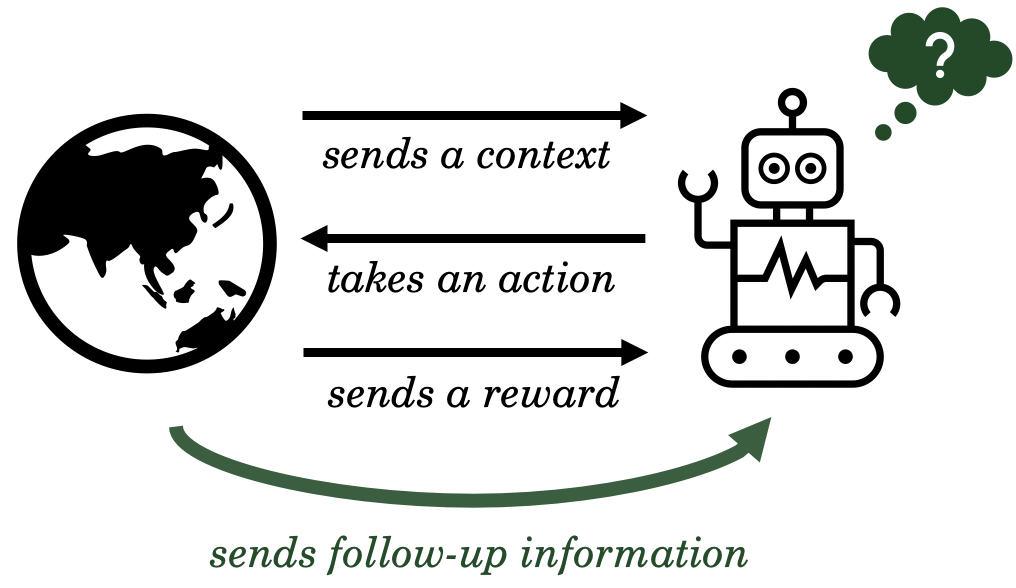
\includegraphics[width=0.5\linewidth]{figs/ex-followup.png}
                \caption{{\small Illustration of learning with post-serving contexts.}}
            \end{figure}
    \end{minipage}

    \vspace{0.5cm} % Space between top and bottom

    % Bottom part for text
    \begin{minipage}[t]{\textwidth}
        \begin{itemize}
            \item \textbf{Motivation}: Post-serving contexts are prevalent in recommender systems.
            \item \textbf{Challenges}: Classical bandit algorithms often fall short in such scenarios.
            \item \textbf{Research question}: How to effectively utilize \textbf{post-serving information} in \textbf{linear contextual bandits}?
        \end{itemize}
    \end{minipage}

\end{frame}
% =======================================

% =======================================
\begin{frame}[label=Background]{Problem Setup and Notations}

\begin{itemize}
    \item \textbf{Problem Setup}: Each time $t = 1, 2, \cdots, T$:
    \begin{itemize}
        \item The learner observes the context $\vx_t$.
        \item The learner selects an arm $a_t \in [K] $.
        \item The learner observes the reward $r_{t,a_t}$.
        \item \textcolor{dgreen}{\textbf{The learner observes the post-serving context $\vz_t$}}.
    \end{itemize}
\end{itemize}


\begin{itemize} \color{gray}
    \item \textbf{Notations}:
    \begin{itemize} \color{gray}
        \item Actions space: $\calA = [K]$.
        
        \item Pre-serving context: $\vx \in \sR^{d_{\vx}}$; post-serving context: $\vz \in \sR^{d_{\vz}}$.
        \begin{itemize} \color{gray}
            \item $\vz = \phi^{\star}\left(\vx_t\right)+\vepsilon_t, \text{and } \phi^{\star}(\vx)=\sE[\vz \mid \vx]$
        \end{itemize}
        
        \item Reward function: 
        \begin{itemize} \color{gray}
            \item $r_{a}(\vx, \vz) = \vx^\top \vtheta_a^\star + \vz^\top \vbeta_a^\star + \eta$, where $\eta$ is $R_{\eta}$-sub-Gaussian.
        \end{itemize}
        
        \item Matrix representation: 
        \begin{itemize} \color{gray}
            \item $\mX_{t} = \sum_{s=1}^t \vx_s\vx_s^\top + \lambda \mI$ and $\mZ_t = \sum_{s=1}^t \vz_s \vz_s^\top + \lambda \mI$.
        \end{itemize}
        
        \item Norm restrictions: 
        \begin{itemize} \color{gray}
            \item $\forall a \in \calA, \|\vtheta_a^\star\|_2\leq 1, \|\vbeta_{a}^\star\|_2\leq 1 $; $\|\vx\|_2\leq L_x, \|\vz\|_2 \leq L_z$.
        \end{itemize}
        
    \end{itemize}
\end{itemize}

\end{frame}
% =======================================


% =======================================
\begin{frame}{Our Contributions}
\begin{itemize}
    \item \textbf{New framework}: 
    \begin{itemize}
        \item Proposed a novel family of contextual bandits with post-serving contexts.
    \end{itemize}
    \item \textbf{Enhanced lemma}: 
    \begin{itemize}
        \item Introduced the Generalized Elliptical Potential Lemma (EPL).
    \end{itemize}
    \item \textbf{Algorithm and theory}: 
    \begin{itemize}
        \item Designed \textbf{\polinucb} with a regret bound of \( \widetilde{\mathcal{O}}(T^{1-\alpha}d_u^{\alpha} + d_u\sqrt{T K })\).
    \end{itemize}
    \item \textbf{Empirical validation}: 
    \begin{itemize}
        \item Achieved SOTA performance on synthetic and real-world datasets.
    \end{itemize}
\end{itemize}
% =======================================


\end{frame}
% =======================================




% %%%%%%%%%%%%%%%%%%%%%%%%%%%%%%%%%%%%%%%
\section{Preliminaries}
% %%%%%%%%%%%%%%%%%%%%%%%%%%%%%%%%%%%%%%%


% =======================================


\begin{frame}{Assumption: Generalized learnability of $\phi^*(\cdot)$}

% TODO: make this more abstract and easily digested by the audience.\\
\begin{alertblock}{Learnability Assumption}
There exists an algorithm that, given $t$ pairs of examples $\{(\vx_s, \vz_s)\}_{s=1}^t$ with  arbitrarily chosen $\vx_s$'s,   outputs an estimated function of $\phi^\star: \mathbb{R}^{d_x} \rightarrow \mathbb{R}^{d_z}$ such that for any $\vx\in \mathbb{R}^{d_x}$,  the following holds with probability at least $1-\delta$, 
\begin{align}
     e_t^\delta:=\left\|\widehat{\phi}_t(\boldsymbol{x})-\phi^{\star}(\boldsymbol{x})\right\|_2 \leq C_0 \cdot\left(\|\boldsymbol{x}\|_{\boldsymbol{X}_t^{-1}}^2\right)^{\textcolor{red}{\alpha}} \cdot \log (t / \delta), \nonumber
\end{align}
where \textcolor{red}{$\alpha \in (0, 1/2]$} and $C_0$ is some universal constant. 
\end{alertblock}

\vspace{+10pt}

\begin{itemize}
    \item The larger the value of $\alpha$, the faster the learning rate for $\phi^{\star}(\cdot)$.
    \item The regret of our algorithm is tied to $O(T^{\textcolor{red}{1-\alpha}})$.
    \item For linear functions, $\alpha = 1/2$ is optimal, yielding a regret of $O(\sqrt{T})$.
\end{itemize}

\end{frame}
% =======================================

% =======================================
\begin{frame}[label=warmup]{Why Natural Attempts May be Inadequate?}
% TODO: WORKING ON THIS.\vspace{+10pt}
\begin{itemize}
    \item Similar to [Wang et al., 2016]~\footfullcite{wang2016learning}, a natural idea is to fit $\widehat{\phi}(\cdot)$, and obtain the parameter estimate by solving:
    {\small
    \begin{align}
    \ell_t (\vtheta_a, \vbeta_a) = \sum_{s\in [t]: a_s = a}  \left(r_{s, a} - \vx_t^\top \vtheta_{a} - \textcolor{red}{\widehat{\phi}_{s}(\vx_s)}^\top \vbeta_{a}\right)^2+\lambda \left( \|\vtheta_a\|_2^2 +  \|\vbeta_a\|_2^2 \right). \nonumber
    \end{align}
    }
    \begin{itemize}
        \item The regret can be $\widetilde{\mathcal{O}}({T^{3/4}})$ when initialized away from the global optimum.
    \end{itemize}
    \vspace{+6pt}
    \item We propose to get the parameter estimate by solving:
    {\small
    \begin{align}\label{eqn:w-closed-form}
    \ell_t (\vtheta_a, \vbeta_a) &= \sum_{s\in[t]: a_s = a}  \left(r_{s, a} - \vx_s^\top \vtheta_{a} - {\color{red}{\vz_s}}^{\top} \vbeta_{a}\right)^2+\lambda \left(\|\vtheta_a\|_2^2 + \|\vbeta_{a}\|_{2}^{2}\right). \nonumber
    \end{align}
    }  
    \begin{itemize}
        \item This requires modification over the original Elliptical Potential Lemma (EPL) to accommodate noise in contexts during learning.
    \end{itemize}
\end{itemize}


\end{frame}
% =======================================

% %%%%%%%%%%%%%%%%%%%%%%%%%%%%%%%%%%%%%%%
\section{Method}
% %%%%%%%%%%%%%%%%%%%%%%%%%%%%%%%%%%%%%%%



% =======================================
\begin{frame}{The Proposed Lemma: Generalized EPL}
\begin{alertblock}{Generalized Elliptical Potential Lemma\footnotemark}
Suppose (1) $\mX_0 \in \mathbb{R}^{d \times d}$ is any positive definite matrix; (2) $\vx_1, \ldots, \vx_T \in \mathbb{R}^d$ and $\max_t \|\vx_t\| \leq L_x$; (3) $\vepsilon_1, \ldots, \vepsilon_T \in \mathbb{R}^d$ are independent bounded zero-mean noises satisfying  $\max_{t} \|\vepsilon_t\| \leq L_{\epsilon}$ and $   \expect[\vepsilon_t \vepsilon_t^\top] \succcurlyeq \sigma^2_{\epsilon} \mI$; %(4)  $\varphi: \mathbb{R}^D \to \mathbb{R}^d$ is a convex context mapping function; 
and (4) $\widetilde{\mX}_t$ is defined as:
{\small
\begin{equation*}\label{eq:data-matrix-GEPL}
    \textcolor{red}{\widetilde{\mX}_t}=\mX_0+\sum_{s=1}^t  (\vx_s \textcolor{red}{\ + \ \vepsilon_s})  (\vx_s \textcolor{red}{\ + \ \vepsilon_s})^{\top} \in \mathbb{R}^{d \times d}. 
\end{equation*} }
For any $p \in [0, 1]$, the following inequality holds with probability at least $1-\delta$,
{\small
\begin{align}\label{eq:gepl-bound}
    \sum_{t=1}^T\left(1 \wedge\left\| \vx_t \right\|_{\textcolor{red}{\widetilde{\mX}_{t-1}^{-1}}}^2\right)^p &\leq \emphgreen{ 2^p T^{1-p}\log^p\left(\frac{\det \mX_T}{\det\mX_0}\right)} \nonumber \\ &\textcolor{gray}{+  \frac{  8 L_\epsilon^2 (L_\epsilon + L_x)^2 }{\sigma_{\epsilon}^4} \log\left(\frac{32d L_\epsilon^2 (L_\epsilon + L_x)^2 }{\delta \sigma_{\epsilon}^4}\right)}.  \nonumber
\end{align}}
\vspace{+0.1pt}
\end{alertblock}
\footnotetext{The original EPL corresponds to the specific case of $p=1$.}

\end{frame}
% =======================================

% =======================================
\begin{frame}{The Proposed Algorithm: \polinucb}
\vspace{-6pt}
\begin{center}

\scalebox{0.85}{\begin{minipage}[c][0.4\paperheight][c]{1.2\textwidth}
  \centering
\begin{algorithm}[H]
\caption{\polinucb~(Linear UCB with post-serving contexts)}\label{alg:polinucb}
\begin{algorithmic}[1]
    % \textbf{Input:} Text Document.\newline
    % \textbf{Output:} Summary sentences.
    % \State{Initialize parameters $\left\{\boldsymbol{A}_{i, 0} \leftarrow \mathbf{I}^d, \boldsymbol{b}_{i, 0} \leftarrow \mathbf{0}^d\right\}$ for all $i \in[K]$ and $\alpha \in \mathbb{R}^{+}$.}
    \For{$t=0, 1, \ldots, T$}
        \State Receive the pre-serving context $\vx _{t}$.
        \State Compute the optimistic parameters by maximizing the UCB objective:
        $${\left(a_t, {\widetilde{\phi}_{t}(\vx_t)}, \widetilde{\vw}_t\right) = {\underset{(a, \phi, \vw_a) \in [K] \times \calC_{t-1}\left(\widehat{\phi}_{t-1}, \vx_t\right) \times \calC_{t-1}(\widehat{\vw}_{t-1,a})  }{\argmax}} { \begin{bmatrix} \vx_t \\ \phi(\vx_t) \end{bmatrix}^\top \vw_{a} }}.$$ 
        \State Play the arm $a_t$ and receive the post-serving context  $\vz_t$ and  the reward $r_{t, a_t}$.
        \State Compute $\widehat{\vw}_{t,a}$ for each $a \in \calA$ using:
        $$\emphgreen{
        \ell_t\left(\boldsymbol{\theta}_a, \beta_a\right)=\sum_{s \in[t]: a_s=a}\left(r_{s, a}-\boldsymbol{x}_s^{\top} \boldsymbol{\theta}_a-\textcolor{red}{\vz_s}^{\top} \beta_a\right)^2+\lambda\left(\left\|\boldsymbol{\theta}_a\right\|_2^2+\left\|\beta_a\right\|_2^2\right)}.
        $$
        \State Compute the estimated post-serving context generating function $\widehat{\phi}_t(\cdot)$ using ERM. 
        \State Update confidence sets $\calC_t(\widehat{\vw}_{t, a})$ and $\calC_t(\widehat{\phi}_t, \vx_t)$ for each $a$.
    \EndFor

\end{algorithmic}
\end{algorithm}
\end{minipage}
}
\end{center}
\end{frame}
% =======================================


% %%%%%%%%%%%%%%%%%%%%%%%%%%%%%%%%%%%%%%%
\section{Results}
% %%%%%%%%%%%%%%%%%%%%%%%%%%%%%%%%%%%%%%%
% =======================================
\begin{frame}{Regret Analysis}

\begin{table}[]
\centering
\begin{tabular}{@{}ll@{}}
\toprule
\textbf{Settings}  & \textbf{Ours} \\ \midrule
Ours               & $\widetilde{\mathcal{O}}\left(T^{1-\alpha}d_u^{\alpha} + d_u\sqrt{T K }\right)$           \\
Action-dependent contexts   & $\widetilde{\mathcal{O}}\left(T^{1-\alpha}d_u^{\alpha}\sqrt{K} + d_u\sqrt{T K }\right)$            \\
Same setting as in [Abbasi et al., 2011]~\footfullcite{abbasi2011improved} & $\widetilde{\mathcal{O}}\left(T^{1-\alpha}d_u^{\alpha} + d_u\sqrt{T  }\right)$            \\ \bottomrule
\end{tabular}
\caption{Upper bound of regret of \polinucb.}
\label{tab:regret}
\end{table}
\end{frame}
% =======================================

% =======================================
\begin{frame}{Experimental Results}

\begin{itemize}
    \item  Our proposed~\polinucb~consistently outperforms other strategies\\\textcolor{gray}{{\footnotesize (except for \texttt{LinUCB} ($x$ and $z$) which equips with post-serving contexts in arm selection)}}.
\end{itemize}

\begin{figure}[h]
    \centering
    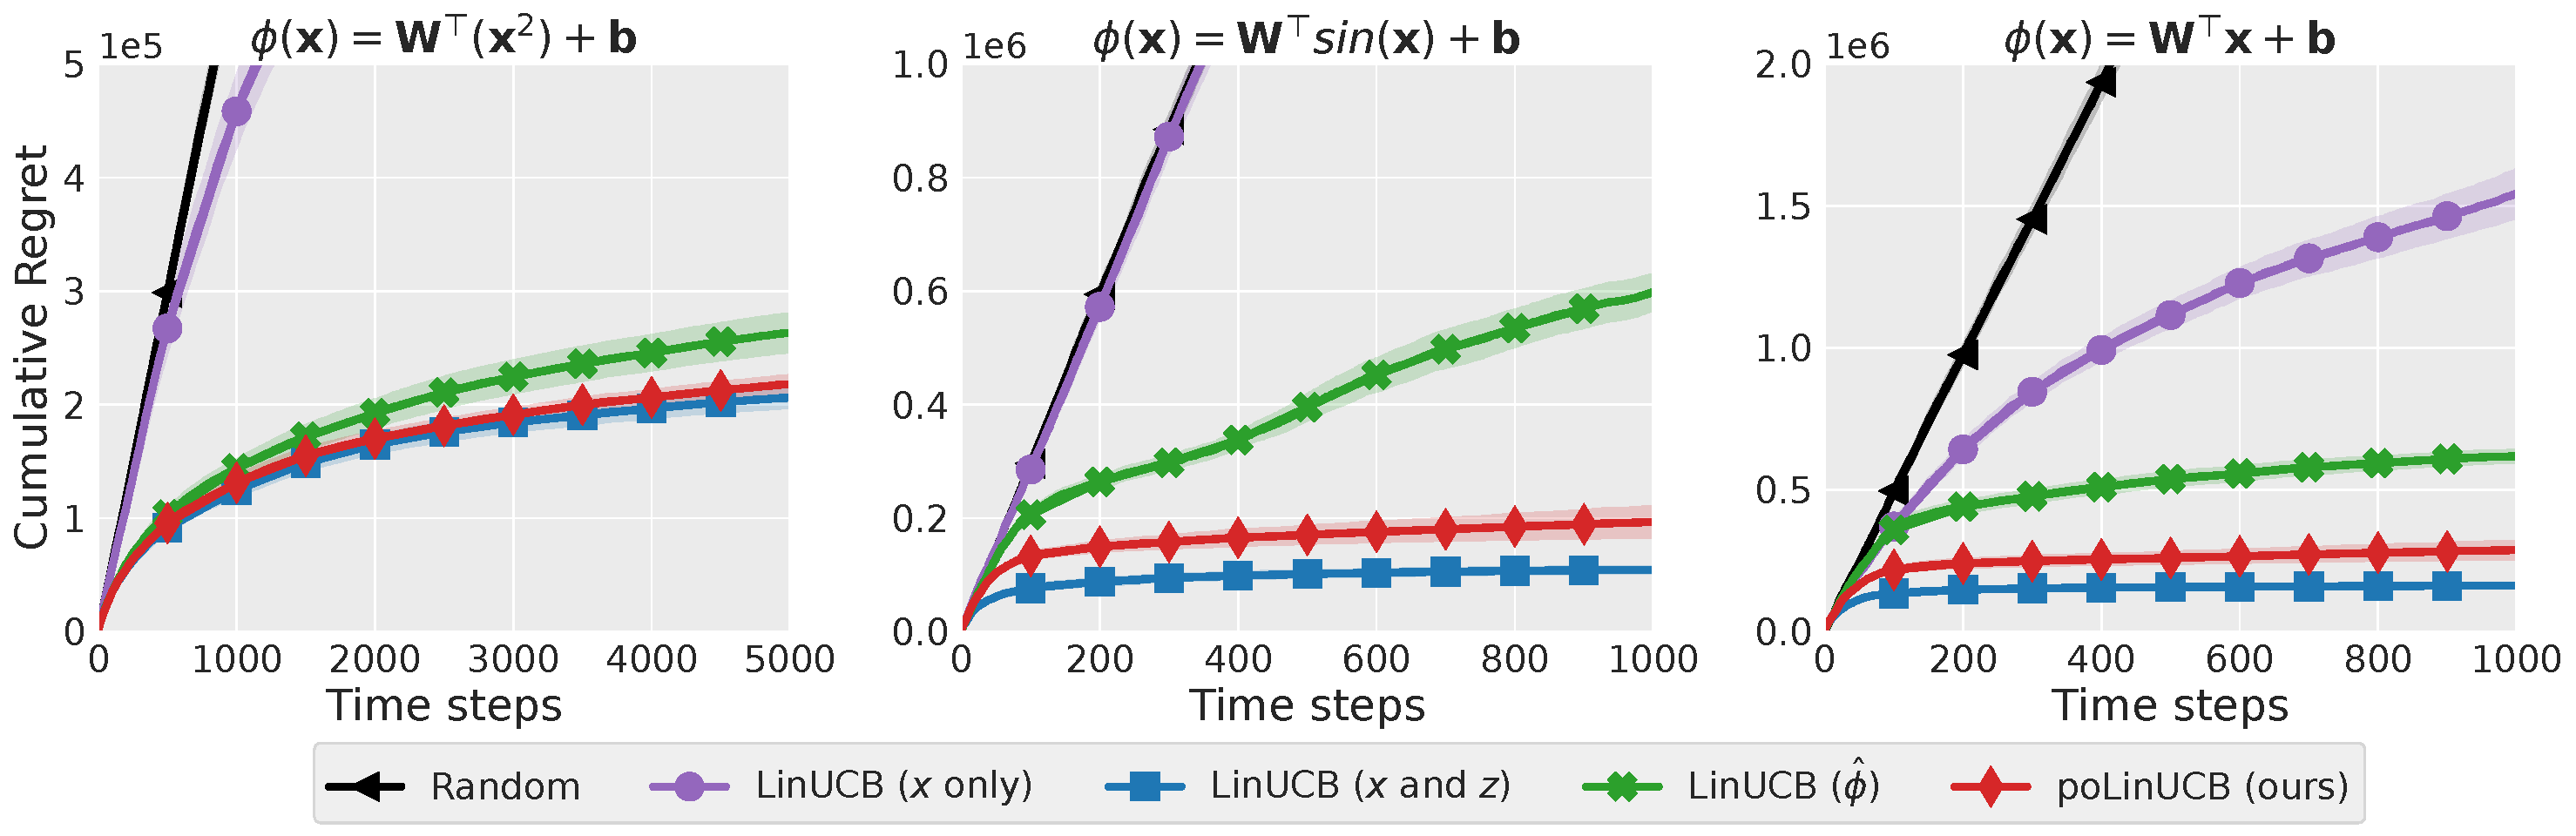
\includegraphics[width=0.85\textwidth]{figs/synthetic-comparisons.pdf}
    \vspace{0.2cm}
    \caption{{\small Cumulative Regret in three synthetic environments. The shaded area denotes the standard error computed using 10 different random seeds.}}
    \label{fig:synthetic-experiments}
\end{figure}

\end{frame}
% =======================================

% =======================================
\begin{frame}
 \begin{center}
		{\Huge \qquad \ \ Thank you.}
		\bigskip\bigskip % Vertical whitespace
  \newline
        \bigskip Please refer to our paper for more information:\\
        \href{https://arxiv.org/abs/2309.13896}{https://arxiv.org/abs/2309.13896}.
	\end{center}
\end{frame}
% =======================================

\end{document}